\documentclass[12pt, titlepage]{article}

\usepackage{booktabs}
\usepackage{tabularx}
\usepackage{hyperref}
\usepackage{graphicx}
\graphicspath{ {./} }
\hypersetup{
    colorlinks,
    citecolor=black,
    filecolor=black,
    linkcolor=red,
    urlcolor=blue
}
\usepackage[round]{natbib}

\title{SE 3XA3: Software Requirements Specification\\Ratava}

\author{Team 9, Makiam Group
		\\ Aidan McPhelim - mcpheima
		\\ Alexie McDonald - mcdona16
		\\ Illya Pilipenko - pilipeni
}

\date{\today}

%\input{../Comments}

\begin{document}

\maketitle

\pagenumbering{roman}
\tableofcontents
\listoftables
\listoffigures

\begin{table}[bp]
\caption{\bf Revision History}
\begin{tabularx}{\textwidth}{p{3cm}p{2cm}X}
\toprule {\bf Date} & {\bf Version} & {\bf Notes}\\
\midrule
2018-10-03 & 1.0 & Created initial Draft, added F and NF requirements\\
2018-10-05 & 1.1 & Filled in the remaining sections\\
2018-10-05 & 1.2 & Finalized formatting\\
2018-12-03 & 1.3 & Updated team name\\
2018-12-05 & 1.4 & Removed old use cases 3, 5, 7, 8\\
\bottomrule
\end{tabularx}
\end{table}

\newpage

\pagenumbering{arabic}

This document describes the requirements for Ratava.  The template for the Software
Requirements Specification (SRS) is a subset of the Volere
template~\citep{RobertsonAndRobertson2012}.  If you make further modifications
to the template, you should explicity state what modifications were made.

\section{Project Drivers}

\subsection{The Purpose of the Project}
Internet avatars became prevalent several years ago in online forums. They were originally not a part of standard practice, but were added in order to personalize responses and provide a sense of identity.

The purpose of this project is to give users a program which can generate unique Avatars for them based on a string of their choosing, which will allow them to share it with their friends if they wish.


\subsection{The Stakeholders}

\subsubsection{The Client}
Since the Professor and TA's of the class want their students to be successful and for the class to do well, they can be considered stakeholders for the software.

\subsubsection{The Customers}
The customers will be internet users at large. Users of social media websites, forums, instant messaging clients to name a few will make good use of an implementation that addresses this problem.

\subsubsection{Other Stakeholders}
There are no further stakeholder apparent for this project.

\subsection{Mandated Constraints}
The main constraint we have is the time constraint - in that we need to have the entire project done with all accompanying documentation by December the 5th.

\subsection{Naming Conventions and Terminology}
Below is a glossary of terms used throughout the specification document
\begin{table}[h!]
\caption{Glossary of terms}
\label{t}
\begin{tabular}{|l|p{10cm}|}
\hline
Word/Phrase & Definition                                                                             \\ \hline
Colour set  & The colours selected to colour regions of the avatar                                   \\ \hline
Item set    & The templates of items that look like every day items (e.g. sword, apple)              \\ \hline
Template    & An image that shows what pixels will be filled where                                   \\ \hline
Hash code   & The output from a hash function (usually a string or hexadecimal)                      \\ \hline
Avatar      & An icon used by an individual to identify themselves in a (typically) online community \\ \hline
\end{tabular}
\end{table}

\subsection{Relevant Facts and Assumptions}
Users of the program are most likely going to be people who are used to computers and play games etc. but when designing the program and UI we will assume that users have no prior knowledge of the terminology involved.



\section{Functional Requirements}

\subsection{The Scope of the Work and the Product}
\subsubsection{The Context of the Work}
\begin{figure}[h]
  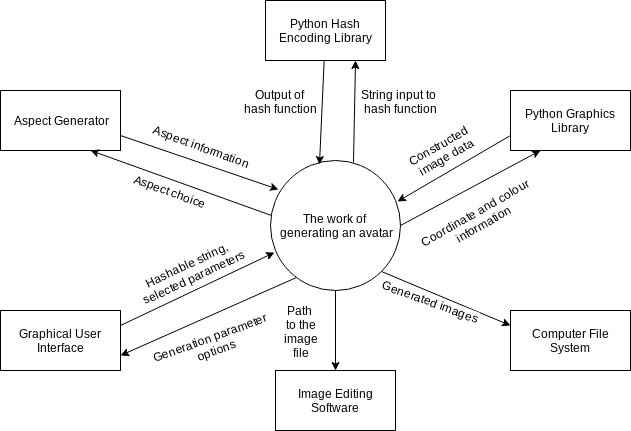
\includegraphics[scale=0.7]{3xa3contextdiagram}
  \caption{Context diagram}
  \label{fig:context}
\end{figure}
\newpage
\subsubsection{Work Partitioning}
\begin{table}[h!]
\caption{Work Partitioning Table}
\label{wpt}
\begin{tabular}{|p{4cm}|p{4cm}|p{8cm}|}
\hline
Event Name & Input and Output & Summary \\ \hline
      User enters seed string   &     input string (in)           &    Record the seed string in a variable within the program  \\ \hline
	User selects template & template key(in) & Set the value of the template variable to the template for the key specified \\ \hline
	User presses generate button & start generation signal(in) & Software begins generation process by triggering the hash function event \\ \hline
	Hash function event triggered & input string variable value (in), hash code (out) & Software passes input string to hash function and records output \\ \hline
       Colour generation by hash code & hash code(in), hexadecimal colour code(out) & Software appends components of the hash code, then converts to hexadecimal to use for the colours \\ \hline
	Weapon generation by hash code portion & hash code (in), weapon pattern (out) & Software uses the first two numeric values of the hash code to index an element in the weapons array \\ \hline
	Picture assembly by property input & template(in), colour mapping(in), weapon key(in), image data(out) & Software passes the coordinate fill information from the template, colour values, and weapons to generate the image file\\ \hline
	Program writes file to file system & image data(in), image file(out) & Software writes the image data to a file in the desired location in the file system \\ \hline
\end{tabular}
\end{table}
\newpage
\subsubsection{Individual Product Use Cases}
\begin{table}[h]
\caption{Use Case Table}
\label{uc}
\begin{tabular}{|p{2cm}|p{9cm}|p{5cm}|}
\hline
Actor & Actor's Goal                                                                                        & Use Case Name                \\ \hline
User  & To generate an avatar with all parameters set at random                                             & GenCompleteRand (UC-1)       \\ \hline
User  & To generate an avatar of a specific template with all other parameters set at random                & GenRandLessTemp (UC-2)       \\ \hline
User  & To generate an avatar of a specific template and colour set with all other parameters set at random & GenRandLessTempColour (UC-3) \\ \hline
User  & To generate an avatar of a specific colour set with all other parameters set at random              & GenRandLessColour (UC-4)     \\ \hline
\end{tabular}
\end{table}
\begin{enumerate}
\item{\textbf{Product Use Case Name:} GenCompleteRand (UC-1) }
\begin{itemize}
\item{\textbf{Trigger:} User presses generate button}
\item{\textbf{Preconditions:} N/A}
\item{\textbf{Interested stakeholders:} The user}
\item{\textbf{Actor:} User}
\item{\textbf{Outcome:} The avatar is generated with no parameters predetermined}
\end{itemize}
\item{\textbf{Product Use Case Name:}  GenRandLessTemp (UC-2)}
\begin{itemize}
\item{\textbf{Trigger:} User presses generate button $\land$ User selects template}
\item{\textbf{Preconditions:} N/A}
\item{\textbf{Interested stakeholders:} The user}
\item{\textbf{Actor:} User}
\item{\textbf{Outcome:} The avatar is generated with the selected template and no other parameters predetermined}
\end{itemize}
\item{\textbf{Product Use Case Name:} GenRandLessTempColour (UC-3)}
\begin{itemize}
\item{\textbf{Trigger:} User presses generate button  $\land$User selects property to fix  $\land$ User selects template}
\item{\textbf{Preconditions:} N/A}
\item{\textbf{Interested stakeholders:} The user}
\item{\textbf{Actor:} User}
\item{\textbf{Outcome:} The avatar is generated with the selected template, selected colour set, and no other parameters predetermined}
\end{itemize}
\item{\textbf{Product Use Case Name:} GenRandLessColour (UC-4) }
\begin{itemize}
\item{\textbf{Trigger:} User presses generate button $\land$ User selects property to fix}
\item{\textbf{Preconditions:} N/A}
\item{\textbf{Interested stakeholders:} The user}
\item{\textbf{Actor:} User}
\item{\textbf{Outcome:} The avatar is generated with the selected colour set, and no other parameters predetermined}
\end{itemize}
\end{enumerate}
\subsection{Functional Requirements}
\begin{itemize}
\item{R1 : Software shall output an image of type .jpg}
\begin{itemize}
\item{\textbf{Fit Criteria:} The resulting file is a lossy graphics file, the extention is .jpg, and it can be opened given the file extension}
\end{itemize}
\item{R2 : Software shall use a hash function to randomize colours and items}
\begin{itemize}
\item{\textbf{Fit Criteria:} The resulting output of the hash function is classified as a hash function of the encoding specified that has the following properties: Compression, strong collision resistance, and the one-way property}
\end{itemize}
\item{R3 : Software shall allow user to select what qualities to fix (and by extention, what qualities to randomize)}
\begin{itemize}
\item{\textbf{Fit Criteria:} The qualities set prior to generation are preserved in the result}
\end{itemize}
\item{R4 : Software shall allow user to select an avatar template}
\begin{itemize}
\item{\textbf{Fit Criteria:} The template set prior to generation is preserved in the result}
\end{itemize}
\item{R5 : Software shall take to a string as input that is used to seed the hash function}
\begin{itemize}
\item{\textbf{Fit Criteria:} The string seeded produces a consistent result with the given hash encoding}
\end{itemize}
\item{R6 : Software shall allow the user to select what hash function that is being used to randomize the elements}
\begin{itemize}
\item{\textbf{Fit Criteria:} The hash function selected, when given the input string, produces the same output as used in the program}
\end{itemize}
\item{R7 : Software shall allow the user to specify the output path}
\begin{itemize}
\item{\textbf{Fit Criteria:} The string representing the location of the file and the string the user entered to determine the location are equal}
\end{itemize}
\item{R8 : Software shall save the image in the location that the user specifies}
\begin{itemize}
\item{\textbf{Fit Criteria:} Indexing into that location in the file system allows the user to locate and open the output file}
\end{itemize}
\item{R9 : Software shall provice access the help documentation}
\begin{itemize}
\item{\textbf{Fit Criteria:} The help implementation can be opened and read in its entirety}
\end{itemize}
\item{R10 : Software shall open the image instantly in an external image editor upon user's request}
\begin{itemize}
\item{\textbf{Fit Criteria:} An image editor opens within 0.5 seconds of the request with the output file in it}
\end{itemize}
\item{R11 : Software shall allow the user to modify the name of the output file}
\begin{itemize}
\item{\textbf{Fit Criteria:} The name provided by the user and the name of the output file are equal}
\end{itemize}
\end{itemize}

\section{Non-functional Requirements}

\subsection{Look and Feel Requirements}
\subsubsection{Accessiblity}
\begin{itemize}
\item{R12 : The software shall implement accessible fonts. That would entail fonts that are sans-serif, simple, and highly legible}
\begin{itemize}
\item{\textbf{Fit Criteria:} All guidelines in the Web Content Accessibility Guidelines are fulfilled to at least the A standard \cite{ontario.ca}}
\end{itemize}
\item{R13 : The user interface elements (buttons, text) should have a high contrast with the background, to aid colour-blind users}
\begin{itemize}
\item{\textbf{Fit Criteria:} Ensure the standards outlined in the World Wide Web Consortium for colour contrast and accessibility are met}
\end{itemize}
\item{R14 : The user interface shall be compatible with a screen reader to aid those who are visually impaired}
\begin{itemize}
\item{\textbf{Fit Criteria:} The running of a screen reader program produces a result that is clear and understandable}
\end{itemize}
\item{R15 : The software shall use intuitive keystrokes throughout the user interface to the meaning of certain operations can be inferred.}
\begin{itemize}
\item{\textbf{Fit Criteria:} A test of the system with a user who did not consult the help documentation yields success when the user is asked to fulfill all use cases of the system}
\end{itemize}
\end{itemize}
\subsection{Usability and Humanity Requirements}
\subsubsection{Ease of Use}
\begin{itemize}
\item{R16 : User interface will be simple, so people who are 8 or above will be able to use it.}
\begin{itemize}
\item{\textbf{Fit Criteria:} 85\% of users who attempt to use the software (out of a statistically random sample) can use the software with little difficulty}
\end{itemize}
\end{itemize}
\subsubsection{Ease of Learning}
\begin{itemize}
\item{R17 : Any user with basic knowledge of a computer's file system will be able to learn this software}
\begin{itemize}
\item{\textbf{Fit Criteria:} 85\% of people who read the help documentation and fulfil the above criterion can use the software with ease}
\end{itemize}
\end{itemize}
\subsection{Performance Requirements}
\subsubsection{Speed Requirements}
\begin{itemize}
\item{R18 : The algorithm used to generate should minimize wait times for the user}
\begin{itemize}
\item{\textbf{Fit Criteria:} The trace of the algorithm should be proven through optimization to be the shortest possible route}
\end{itemize}
\item{R19 : The program at most should take no longer than 5 seconds maximum. A study performed in 1995 says that 10 seconds is a tolerable wait time for a web response. Moreover, 1 second is the limit for the user's train of thought to flow continously. \cite{nielsen_1995}}
\begin{itemize}
\item{\textbf{Fit Criteria:} The difference in the moment the generator button is pressed and the result becomes avaliable in the file system should be no greater than 5 seconds}
\end{itemize}
\end{itemize}
\subsubsection{Precision Requirements}
\begin{itemize}
\item{R20 : Pixels displayed to the user shall exactly match the pixel placement outlined in the templates}
\begin{itemize}
\item{\textbf{Fit Criteria:} $\forall a \in template \land b \in output \bullet a(x,y) = b(x,y)$}
\end{itemize}
\end{itemize}
\subsubsection{Reliability and Avaliability}
\begin{itemize}
\item{R21 : The software will be operable 24hrs a day, 7 days a week, 365 days a year, Due to the program being on a local machine with no dependency on any external resources other than a working file system and python compiler.}
\begin{itemize}
\item{\textbf{Fit Criteria:} An ongoing stress test of the system for the time specified above yields no blackouts or interuptions}
\end{itemize}
\end{itemize}
\subsubsection{Capacity Requirements}
\begin{itemize}
\item{R22 : The software shall have an ultimited amount of concurrent users on unique machines, Due to the program being on a local machine.}
\begin{itemize}
\item{\textbf{Fit Criteria:} Have 10 users use the program concurrently and record the difference in time to only one person running it}
\end{itemize}
\item{R23 : The software shall have a limit of one concurrent user per machine.}
\begin{itemize}
\item{\textbf{Fit Criteria:} Attempts to have two users use the same program concurrently fail}
\end{itemize}
\end{itemize}
\subsubsection{Expected Technological Environment}
\label{sec:ETE}
\begin{itemize}
\item{R24 : The expected technological environment will ultimately be a computer that is running an operating system that can support usage of a python3 compiler and interpreter, and has a traditional file system.}
\begin{itemize}
\item{\textbf{Fit Criteria:} Download a selection of the most popular virtual machine environments and ensure the software runs on each}
\end{itemize}
\end{itemize}
\subsubsection{Partner Applications}
\begin{itemize}
\item{R25 : There is no partner applications that the software will need to interface with.}
\begin{itemize}
\item{\textbf{Fit Criteria:} N/A}
\end{itemize}
\end{itemize}
\subsection{Maintainability and Support Requirements}
\subsubsection{Mainainability}
\begin{itemize}
\item{R26 : The software shall support the addition of new templates at a later date}
\begin{itemize}
\item{\textbf{Fit Criteria:} An addition of a new template after software release fails to change program behaviour negatively}
\end{itemize}
\item{R27 : The software shall support the addition of new hash functions at a later date}
\begin{itemize}
\item{\textbf{Fit Criteria:} An addition of a new hash encoding after software release fails to change program behaviour negatively}
\end{itemize}
\item{R28 : The software shall support the addition of new elements to the user interface at a later date}
\begin{itemize}
\item{\textbf{Fit Criteria:} An addition of a new user interface element after software release fails to change program behaviour negatively}
\end{itemize}
\item{R29 : The software shall be decomposed into modules with a level of low cohesion that allows them to be serviced without breaking the other modules}
\begin{itemize}
\item{\textbf{Fit Criteria:} The modification of a module after release passes all integration tests}
\end{itemize}
\end{itemize}
\subsubsection{Portability}
\begin{itemize}
\item{R30 : As outlined in \hyperref[sec:ETE]{Section 3.4.5} the software shall run on any operating system that supports the usage of a python compiler, interpreter, and modifications to the files present on the file system}
\begin{itemize}
\item{\textbf{Fit Criteria:} Same as in \hyperref[sec:ETE]{Section 3.4.5}}
\end{itemize}
\end{itemize}
\subsection{Security Requirements}
\begin{itemize}
\item{R31 : The software shall dispose of all strings entered that hashed the functions}
\begin{itemize}
\item{\textbf{Fit Criteria:} A query of the variables/data accessible by the user after run time yields no strings provided}
\end{itemize}
\item{R32 : Randomness of the hash function shall ensure that the hash string cannot be infered from the template it generates}
\begin{itemize}
\item{\textbf{Fit Criteria:} An attempt to reverse the hash function yields a result different from the one entered}
\end{itemize}
\item{R33 : The software shall prevent data interceptions by running as a standalone application on a desktop computer}
\begin{itemize}
\item{\textbf{Fit Criteria:} Attempts at a data interception via any method except unauthorized remote access is unsuccessful}
\end{itemize}
\end{itemize}
\subsection{Cultural Requirements}
\begin{itemize}
\item{R34 : The software shall not use any symbols or imagery for templates that could offend the country using it}
\begin{itemize}
\item{\textbf{Fit Criteria:} Templates, items, and colour sets used do not resemble any content deemed to be sensitive}
\end{itemize}
\end{itemize}
\subsection{Legal Requirements}
\begin{itemize}
\item{R35 : The elements of the software shall support the requirements outlined in the licence underwhich the software is licenced.}
\begin{itemize}
\item{\textbf{Fit Criteria:} Every regulation outlined in the General Public Licence 2.0 documentation is fulfilled \cite{GNU}}
\end{itemize}
\item{R36 : The software shall be compliant with all privacy regulations}
\begin{itemize}
\item{\textbf{Fit Criteria:} Every regulation in the The Personal Information Protection and Electronic Documents Act (PIPEDA) is satisfied \cite{ahmad_tariq_2017}}
\end{itemize}
\end{itemize}
\subsection{Health and Safety Requirements}
Not applicable to this software. \\

This section is not in the original Volere template, but health and safety are
issues that should be considered for every engineering project.

\section{Project Issues}

\subsection{Open Issues}
None have been found so far.

\subsection{Off-the-Shelf Solutions}
There are already similar products available, such as https://robohash.org/, but
string-hash based random avatar generation is a business field where getting
off-the-shelf solutions from other developers for the purpose of using them in
one's own product is a very difficult task.

\subsection{New Problems}
This software main problem that will exist after this software is in place is the restriction on resolution of avatar images. Users can of course still have higher resolution images, but in terms of generating random avatars that are unique to them, they will have to settle for a very low resolution.

\subsection{Tasks}
\begin{itemize}
  \item plan for proof of concept demonstration
  \item create a test plan
  \item design and document revision 0
  \item prepare for revision 0 demonstration
  \item research into pixel art
  \item create the template for software design
  \item start work on the program
\end{itemize}

\subsection{Migration to the New Product}
Since the project's service is simple, discrete, and has data stored only on the
user's side, there are no requirements for migration to the new product, nor does
any data need to be modified or translated for the new system.

\subsection{Risks}
\begin{tabular}{| c | c | c |}
  \hline
  Risk & probability & countermeasure \\
  \hline
  Low productivity & high & implement agile method \\
  \hline
  Excessive schedule pressure & medium & reduce task load, implement agile method \\
  \hline
  Overabundance of features & low & remoe unnecessary features \\
  \hline
\end{tabular}
\subsection{Costs}
As the resources being drawn upon for the creation of this project have no financial cost, the only cost to consider is the cost of time and effort. As outlined before, this project is well within the scope of a semester's worth of work split amongst three students, so the resource cost will be moderate.

\subsection{User Documentation and Training}
\begin{itemize}
  \item User Documentation Requirements:  an opeations manual describing how to
  use the product and what to expect from it should be provided alongside the product.
  \item Training Requirements: no training is needed to use the product.
\end{itemize}

\subsection{Waiting Room}
There are no requirements in the waiting room.

\subsection{Ideas for Solutions}
There are no ideas for solutions.

\bibliographystyle{plainnat}

\bibliography{SRS}

\newpage

\section{Appendix}

This section has been added to the Volere template.  This is where you can place
additional information.

\subsection{Symbolic Parameters}

The definition of the requirements will likely call for SYMBOLIC\_CONSTANTS.
Their values are defined in this section for easy maintenance.


\end{document}
